 \documentclass[conference]{IEEEtran}
\IEEEoverridecommandlockouts
% The preceding line is only needed to identify funding in the first footnote. If that is unneeded, please comment it out.
\usepackage{cite}
\usepackage{amsmath,amssymb,amsfonts}
\usepackage{algorithmic}
\usepackage{graphicx}
\usepackage{textcomp}
\usepackage{xcolor}
\usepackage{algorithm}
\usepackage{algorithmic}
\usepackage{subfig}

\renewcommand{\algorithmicrequire}{\textbf{Input:}} % Use Input in the format of Algorithm
\renewcommand{\algorithmicensure}{\textbf{Output:}} % Use Output in the format of Algorithm

\newcommand{\TheName}{ADGuard}
\newcommand{\TheAttack}{low-rate TCP attack}

\def\BibTeX{{\rm B\kern-.05em{\sc i\kern-.025em b}\kern-.08em
    T\kern-.1667em\lower.7ex\hbox{E}\kern-.125emX}}
\begin{document}

\title{\TheName{}: Adaptively Defend the Low-Rate TCP attack in SDN
}

\author{
\IEEEauthorblockN{Renjie Xie\IEEEauthorrefmark{1}\IEEEauthorrefmark{2}\IEEEauthorrefmark{3}, 
Jiahao Cao\IEEEauthorrefmark{1}\IEEEauthorrefmark{2},
Mingwei Xu\IEEEauthorrefmark{1}\IEEEauthorrefmark{2}, 
Qi Li\IEEEauthorrefmark{1}\IEEEauthorrefmark{2},\IEEEauthorrefmark{3} 
} 

\IEEEauthorblockA{\IEEEauthorrefmark{1}
Department of Computer Science and Technology, Tsinghua University, Beijing, China} 
\IEEEauthorblockA{\IEEEauthorrefmark{2}
Beijing National Research Center for Information Science and Technology(BNRist), Beijing, China} 
\IEEEauthorblockA{\IEEEauthorrefmark{3}
Graduate School at Shenzhen, Tsinghua Univesity, Guangzhou, China}
\IEEEauthorblockA{
\{xrj16, caojh15\}@mails.tsinghua.edu.cn, xumw@tsinghua.edu.cn, 
qi.li@sz.tsinghua.edu.cn}
}

\maketitle

\begin{abstract}
\emph{The low-rate TCP attack} \cite{b20} is essentially a periodic burst which has a big influence on the TCP flows for the retransmission mechanism of TCP. After synchronizing the burst period to the Retransmission Timeout (RTO) duration, the low-rate TCP attack forces the TCP flows to cause retransmission continuously. Because of the low average rate, this sort of attack is difficult to detect. In this paper, we propose an adaptive detection approach \TheName{} which detects the affected port by the periodicity of the attack and classifies flows by the mean Euclidean distance between the normalized signal of the flows and the affected port with Software Defined Networking (SDN). To minimize the influence of the attack, the flow rule can be installed in the access switches to drop all the attack packets from the attack hosts thanks to the global view of SDN. We demonstrate the accuracy and performance of \TheName{} in a real SDN testbed consisting of hardware switches. The experiment results show that \TheName{} accurately detects and effectively defends the low-rate TCP attack.
\end{abstract}

% \begin{IEEEkeywords}
% component, formatting, style, styling, insert
% \end{IEEEkeywords}

\section{Introduction}
DoS (Denial of Service) attacks are a great threat to Internet security. The Internet suffers from the DoS attacks frequently, for example, the most powerful DDoS attack hits the developer platform GitHub with a traffic of 1.35 Tbps on March 1st, 2018 \cite{b19}. DoS attacks are almost flooding-based: TCP SYN flooding, exhausting the system source, and DNS flooding, exhausting the bandwidth, are typical representatives of DoS attacks. \cite{b20} presents \emph{low-rate} TCP attack, in which the attacker sends periodical traffic to overload the bandwidth of a router and leads to packet losses in a link. By synchronizing the attack period to the RTO duration, the low-rate TCP attack induces retransmission of the TCP flows continuously. Detecting the low-rate TCP attack is much more difficult than detecting traditional DoS attacks because of the low average rate. In addition, any router forwarding the TCP flows can be the target of the attack. Moreover, The attack can be launched in a distributed mode, therefore, the attack sources are hard to be located. Once a TCP flow becomes a victim of the low-rate TCP attack, the throughput of the flow will become very low. Hence, the protocols based on TCP are influenced seriously, e.g. HTTP, FTP, and BGP.

Several schemes have analyzed the traffic by exploring \emph{digital signal processing} (DSP) in time domain and frequency domain \cite{b6}, \cite{b7}, \cite{b4}, \cite{b22}, \cite{b1}. By examing the frequency-domain characteristics, \cite{b3} detects the low-rate TCP attack quickly. Other schemes also mitigate the low-rate TCP attack with different mechanisms. \cite{b17} randomized the TCP RTO to counter the low-rate TCP attack, which needs to be deployed in the end host and modifies the default behavior of TCP. \cite{b8} modifies fairness of drop packets in the switches and prevents the low-rate TCP attack by dropping packets. Unfortunately, none of the above defense schemes could adaptively detect the low-rate TCP attack and make deployment easier.

SDN provides new methods to defend against DDoS attacks. Flow information collected from the SDN switches and the global view of the network provided by the SDN controller can be utilized to analyze DDoS attacks. With the support of SDN, the defense system could detect the attack flows, even locate the attack sources. Recently several SDN-based approaches have been proposed to detect and mitigate DDoS \cite{b9}, \cite{b16}, \cite{b11}, \cite{b23}, \cite{b24}. With these approaches, various DDoS attacks are effectively and efficiently detected. However, they fail to detect and defend low-rate TCP attack. The target of low-rate TCP attack is the link of TCP flows' paths, and the average rate of low-rate TCP attack is reduced compared with the other DDoS, hence the low-rate TCP attack is harder to be detected than the flooding style attack.

In this paper, we propose an adaptive approach to detect and mitigate the low-rate TCP attack by analyzing the periodicity of the low-rate TCP attack. If the throughput of TCP flows is reduced in a switch, we monitor all the active ports of the switch. The key to detecting the low-rate TCP attack is to determine the periodicity of the rate data in our approach. To determine the periodicity, we collect the time-domain signal by taking samples of packet arriving rate with decreasing sampling period, and transform it into the frequency domain by FFT (\emph{Fast Fourier Transfrom}) for the constant period of low-rate TCP attack, as the period of the samples can be obtained by analyzing FFT. And then, we compare the statistics of the port detected to be attacked by the low-rate TCP attack with the statistics of the flow rules related the port to detect the attack flows. After the attack flows are detected, we identify the attackers by analyzing the match fields of flow rules forwarding attack traffic and isolate them by installing flow rules to drop packets from the attackers. Our detection minimizes the overhead of the controller by adaptive sampling period. The influence of the low-rate TCP attack is minimized by mitigating the attack in the access switches. Notice that though the low-rate TCP attack is distributed, the attack can be detected and mitigated in our system.

To prove the effectiveness and accuracy of our defense system, we conduct the experiment with a real SDN testbed consist of hardware switches. The experiment results illustrate that the period of the low-rate TCP attack can be inferred during the period are increased from 0.1 s to 1 s in an acceptable error, meanwhile, the attack flows can be detected in an appropriate sampling period. Based on the analysis of more than 1,000 simulations, more than 90\% attack flows can be detected with the increasing period from 0.8s to 1.5s. The throughput with the protection of our system is far higher than that of without protection, meanwhile, it introduces additional 14\% CPU usage at most. To summarize, we make the following contributions:

\begin{itemize}

\item We propose a defense system called \TheName{}, which can effectively defend low-rate TCP attack without any modification in the hardware switches or SDN protocols.  
\item We develop algorithms that can accurately detect the low-rate TCP attack, obtain the appropriate sampling period to determine attack flows for isolating the attackers.
\item We implement \TheName{} in Floodlight controller with real hardware testbed, and successfully defend the low-rate TCP attack, even it is distributed.

\end{itemize}

\section{Background}
In this section, we introduce some background knowledge about the working principle of low-rate TCP attack and counters that help to analyze the flows in SDN.

\subsection{The Low-rate TCP Attack}
The low-rate TCP attack is a periodic burst which has an impact on the TCP flows. We consider the link of a switch with capacity $C$. The periodic square wave is a typical form of the attack in \cite{b20}. We denote the period by $T$, and the burst length of the square wave is $L$ units of time within each period. We denote the ratio $L / T$ by $\eta$. During the burst, the square wave has a peak rate of $R$. Thus the average rate of this form of attack is $\eta R$. During the burst of the attack traffic, the victim switches will be filled up with attack packets so that they discard all the packets of TCP flows. TCP flows are forced to retransmit continuously. Note that $\eta$ should be small to avoid being detected by the high traffic volume.

Figure~\ref{fig:LDoS} illustrates a general model of low-rate TCP traffic which can be described by three parameters ($R, L, T$). Note that either a single source or multiple distributed sources can generate low-rate TCP attack traffic in \cite{b4}. Two approaches for generating a distributed attack are mentioned in \cite{b3}. Supposing that $D$ distributed hosts generate low-rate TCP attack, one method is generating the attack with the same period $T$ and burst rate $R/D$, and the other method is with period $DT$ and burst rate $R$. The low-rate TCP attack traffic is distributed in different attack sources and needs to be synchronized so that the aggregate traffic forms the desired square wave at the targeted link. 

\begin{figure}
\vspace{-0.2in}
\centering
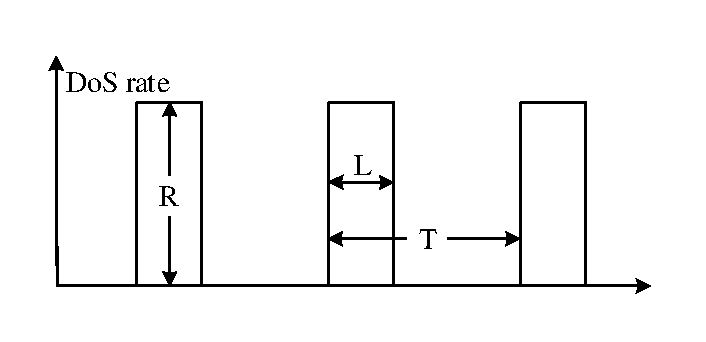
\includegraphics[width=3.4in]{Design/LDoS.pdf}
\vspace{-0.1in}
\caption{\small{Low-rate TCP attack traffic.}}
\label{fig:LDoS}
\vspace{-0.2in}
\end{figure}




\subsection{Counters and Meters of SDN}
In SDN, \emph{counters} are enabled to count the information of the switches, therefore, they help the controller detect the low-rate TCP attack and locate the hosts. Counters are maintained for the bytes of the ports and flow rules. In a switch, a packet is matched by the flow rules and the highest priority flow rule that matches the packet will be selected to deal with the packet, therefore, the counters associated the flow rule will be updated. Moreover, if the packet is transmitted by a port, the counter associated with the port will be updated. Counters can be used to monitor the throughput of flows, locate attack hosts and flow rule. The counters associated with a flow rule matching all the TCP packets are used to collect statistics of the TCP flows in a switch. The counters associated with ports will help to detect the affected ports. The counters associated with forwarding rules will help to locate attack hosts. Considering that we have a sequence of the byte count $B$ with the sampling period $T_b$, the rate signals $R$ of a counter can be obtained by:

\vspace{-0.05in}
\begin{equation}\label{eq:sampling}
\ R_i=\frac{B_i - B_{i - 1}}{T_b}
\end{equation}

\textit{Meters} enable the SDN to implement rate-limiting for flows and ports. The meter controls the rate of the aggregate of all flow rules to which it is attached. Note that, the \emph{burst\_size} defines the granularity of the meter. To mitigate the low-rate TCP attack, the fine-grained meter is required for the low average rate of the attack.

\section{Design}
In this section, we show the three modules of \TheName{}, i.e. \emph{Monitor}, \emph{Locator}, and \emph{Mitigator}. Figure~\ref{fig:architecture} shows the architecture of our design. Monitor collects the aggregated throughput of TCP flows from every switch. Once the throughput of a switch degrades significantly, Locator will be triggered to pull the statistics about the affected ports of the switch to help locate the attack sources. To eliminate the influence of the low-rate TCP attack, Mitigator installs flow rules to drop the attack packets at the access switches of attack sources identified by Locator.


\begin{figure}
\vspace{0in}
\centering
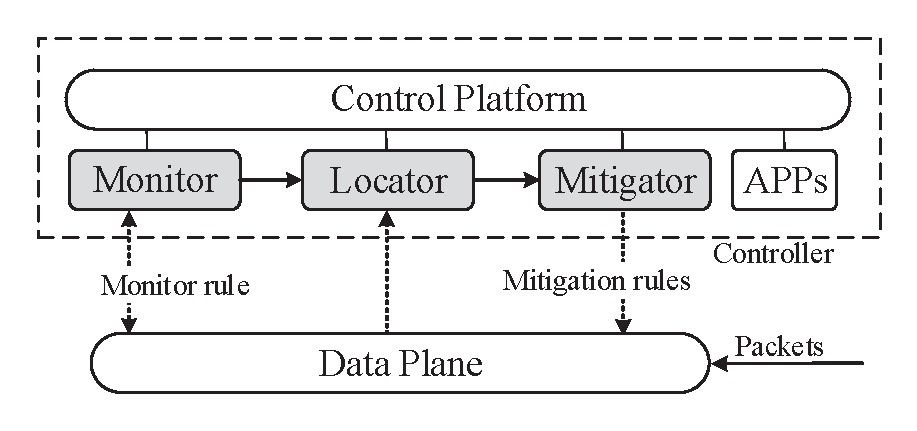
\includegraphics[width=3.4in]{Design/architecture.pdf}
\vspace{-0.1in}
\caption{\small{The architecture of our design.}}
\label{fig:architecture}
\vspace{-0.2in}
\end{figure}


\subsection{Monitor Module}
Monitor is designed to alert the system for the TCP throughput degradation in every switch. To detect the low-rate TCP attack, Monitor needs to track the aggregated throughput of TCP flows. Therefore, Monitor installs flow rules that match the TCP packets with the highest priority in each switch. The flow rules include a Goto-table instruction to guarantee the normal packet transmission, and it is just used to record the aggregated throughput of TCP flows. In a switch, the significant degradation of TCP throughput may be caused by the low rate TCP attack. Thus, Monitor triggers Locator for more accurate detection of the low-rate TCP attack. 

%The module decreases the overhead effectively, as it avoids invalid detection. 

\begin{algorithm}[H]
  \caption{TCP Traffic Monitor}
  \label{alg:match}
  \begin{algorithmic}[1]
  \REQUIRE $M, \alpha, R$;
  \ENSURE $s$;
  \STATE $c \gets 0$;
  \STATE $s \gets not degraded$;
  \FOR{$(i=2 \rightarrow {size(R)})$}
      \IF {$R_{i} < {\alpha} * R_{i - 1}$}
        \STATE $c \gets c + 1$;
    \ELSE 
        \STATE $c \gets 0$;
    \ENDIF
    \IF {$c {\ge} M$}
        \STATE $s \gets degraded$;
    \ENDIF
  \ENDFOR
  \RETURN $s$;
  \end{algorithmic}
\end{algorithm}

Algorithm~\ref{alg:match} shows the pseudo-code of Monitor. The inputs consist of $\alpha$ (the degradation threshold), $R$ (the sequence of aggregated TCP throughput with a chosen sampling period) and $M$ (the threshold for the degradation length). The output is TCP traffic states $s$. First, $c$ is the variable to record the duration of TCP traffic's degradation, and $s$ represents whether the throughput of TCP traffic degrades. Step 1 to Step 2 initializes the $c$ and $s$. Step 4 to Step 11 determines the state of aggregated throughput. To meet the various requirement, the sampling period can be set by the managers. When the significant degradation of aggregated throughput is confirmed, Locator will be triggered for more accurate detection.

\subsection{Locator Module}

Locator aims at confirming the low-rate TCP attack and locating the attack sources. It detects the active ports for the affected port and identifies the attack sources by analyzing the flow rules associated with the affected ports. Considering that the packets, transmitted by the affected port, consist of attack packets and legitimate packets, we apply the thresholding method to filter noise introduced by the legitimate flows. And then, we obtain binary signals of affected port. The periodicity of the binary signals can be used to confirm the low-rate TCP attack. When a port is confirmed to be affected by the attack, we can identify the attack sources by the similarity between the binary signals of the attack flows and that of the affected port.

\noindent \textbf{Signal Binarization.} Note that the collected input includes some packets, besides the potential low-rate TCP attack packets. The TCP packets, surviving from the low-rate TCP attack, and the UDP packets are the noise for the counters associated with the ports. For a clean signal, the thresholding method is applied to filter noise. The peak rate of the signals is $R$. The collected signals no more than $\beta R$ will be clamped to 0, and the others are set to 1. In our system, we set $\beta$ = 0.8.

\noindent \textbf{The Period of Analog Signal and Digital Signal.} Assuming that periodic analog signals with a period of $T$ are sampled with the appropriate sampling period $T_s$, we can get digital signals with a period of $T_b$. $T_b$ can be obtained from the digital signals by FFT because the power of $T_b$ is the maximum value in the power spectrum of the signal.
According to the \emph{Nyquist} theorem (i.e. $T_s \le T/2$), $T$ can be obtained by:

\vspace{-0.05in}
\begin{equation}\label{eq:period}
\ T = T_s * T_b
\vspace{-0.05in}
\end{equation}




For a periodic signal, $T$ obtained by the equation~\ref{eq:period} will be a constant if $T_s$ is small sufficiently. In other words, if the value of $T_s * T_b$ will not change with the decreasing $T_s$, the signal will be a periodic signal. Thus, the clean signals of a port have a constant period of $T$ with decreasing $T_s$, the port is confirmed to be affected by the low-rate TCP attack.

Due to the low-rate TCP attack have the characteristics of low average rate and short periodic burst, the sampling period of detection should be as short as possible. However, the number of packets transmitted from a switch to the controller is limited by the bandwidth of control channel and resources of the switch. According to the above analysis, an appropriate $T_s$ can be used to detect attacks with the minimized overhead for the system. 

To locate the attack hosts, the port affected by the low-rate TCP attack should be detected first. Hence, we design an adaptive algorithm for the active ports.

\begin{algorithm}[H]
  \caption{Affected Port Detection}
  \label{alg:port_locate}
  \begin{algorithmic}[1]
  \REQUIRE $~{\epsilon}, p, T_{min}, T_{max}$;
  \ENSURE $s, T_s, T$;
  \STATE $T_s \gets T_{max}$;
  \STATE $T \gets \infty$; 
  \WHILE{$T_s \ge T_{min}$}
      \STATE $signal \gets binary\_signal(T_s, p)$;
      \STATE $T_b \gets period\_mean\_fft(signal)$;
      \IF {$abs(T - T_b * T_s)<\epsilon$}
            \STATE $s \gets$ \emph{affected};
              \RETURN $s, T_s, T$;
        \ELSE
          \STATE $T \gets T_b * T_s$;
          \STATE $T_s \gets T_s / 2$;
      \ENDIF 
  \ENDWHILE
  \STATE $s \gets$ \emph{not~affected};
  \STATE $T \gets 0$; 
  \RETURN $s, T_s, T$;
  \end{algorithmic}
\end{algorithm}

The pseudo-code of locating the affected ports is shown in Algorithm~\ref{alg:port_locate}. The inputs consist of accepted error of period $\epsilon$, the detected port $p$, the lower bound of sampling period $T_{min}$, and the upper bound of sampling period $T_{max}$. The outputs consist of port state $s$, the appropriate sampling period $T_s$, and inter-burst period $T$. Step 1 initializes $T_s$ with $T_{max}$. Step 2 sets $T$ to infinity because the period of signals associated with the port is unknown at the beginning. The main loop is from Step 3 to Step 13. In each loop iteration, the algorithm tests $T_s$. Step 4 achieves the coming rate of $p$ with sampling period $T_s$, and generates $signal$ by binarizing it. In Step 5, the algorithm gets the period of $signal$ by analyzing FFT. Step 6 to Step 8 compare the periods of the $signal$ with decreasing sampling period. If the difference of them is smaller than $\epsilon$, the port will be confirmed to be affected by the low-rate TCP attack. Moreover, the inter-burst period of the attack is $T$ with the sampling period $T_s$. Otherwise, the frequency of sampling will be doubled, and set $T$ to be the current measured period (Step 9 to Step 11). Step 14 to Step 16 set $T_b$ to be infinity and the port is not affected by the attack. The period of the analog signal and digital signal are described by Equation~\ref{eq:period} with appropriate sampling period $T_s$. Thus, Algorithm~\ref{alg:port_locate} calculates $T$ with decreasing sampling period until $T$ is obtained or $T_s$ is less than $T_{min}$. Note that $T_s$ is used for the next steps instead of a constant period, which means the attack with the short period cannot survive from the detection and the attack with long period introduces less overhead.


\noindent \textbf{Sequence-Similarity.} Once the affected port is confirmed, the analysis of flows are required for locating the attackers. The similarity between the binary signals of flows and that of the affected port can be used to detect attack flows. For the sampling period of $T_s$ obtained from above algorithm, we denote the binary signals of the affected port as $A$ and the binary signals of a flow rule associated with the port as $B$. Supposing that $A$ and $B$ are obtained at the same time. Mean Euclidean Distance (MED) of $A$ and $B$ represents the similarity between $ A $ and $B$, and it can be calculated by:

\vspace{-0.05in}
\begin{equation}\label{eq:euclidean_distance}
\ MED=\frac{\sum_{i=1}^{N}\lvert A_{i} - B_{i}\rvert}{N}.
\vspace{-0.05in}
\end{equation}

The binary signals of low-rate TCP attack flows are more similar to the that of affected ports than others. Thus, the MED of low-rate TCP attack flows is smaller than that of the legitimate flows. A binary classifier can be used for the flows. We set a threshold $\gamma$ for the classifier. The flows, whose MED is less than $\gamma$, will be classified to attack flows. Note that either the single source or multiple distributed sources can be detected for the flow-level detection. Thanks to the global view of SDN, the attack sources can be located for mitigation.

\subsection{Mitigator Module}

The purpose of this module is mitigating the low-rate TCP attack. Note that the attack sources, i.e. hosts, access the SDN network directly or through an unknown network. For the first case, we mitigate the attacks by installing block flow rules for access ports in the access switches. As for the second case, the match field includes more information besides the ports information. 

we propose two methods for mitigation, dropping the packets and limiting the bandwidth. For the first method, the flow rules, which match the attack hosts with the highest priority, will be installed in the access switches of the attack sources. These rules will drop all the attack traffic. The attack packets cannot be injected into the network anymore with the first method. Therefore, the influence of the attack will be eliminated. However, some legitimate traffic may be affected by the erroneous decision made by Locator. We leverage meter entries for rate limitation in the second method. Mitigator will assign all the flow rules confirmed to transmit the attack traffic. Note that the low-rate TCP attack has a high rate only during the burst. Thus, The meter with coarse-grained fails to limit the attack because of the low average rate. For the suitable granularity of meters, the burst\_size is set based on $T_s$.

Figure~\ref{fig:mitigate} shows that the mechanism of the first method in the first case. The attacker $h_1$ access the network at port 1 and the legitimate user $h_2$ access the network at port 2 in the switch $S_1$. In addition, they both send packets to the server. The attacker is desired to overload the bandwidth of the link between $S_1$ and $S_2$ and causes retransmission of the TCP flows between $h_2$ and server. After Mitigator installs flow rules for the attacker, the packets $h_1$ are dropped in $S_1$, and the packets from $h_2$ are transmitted through the path. 

To meet the various performance requirements, the network managers can determine which method is used in the system. In general, the first method is a better way to mitigate the low-rate TCP attack. However, under the circumstances where the managers desire to reserve bandwidth for all the hosts, the second method is more suited to mitigate the attack. The default method of our system is dropping all the packets from the attack hosts for the security of the network. 



\begin{figure}
\vspace{-0.2in}
\centering
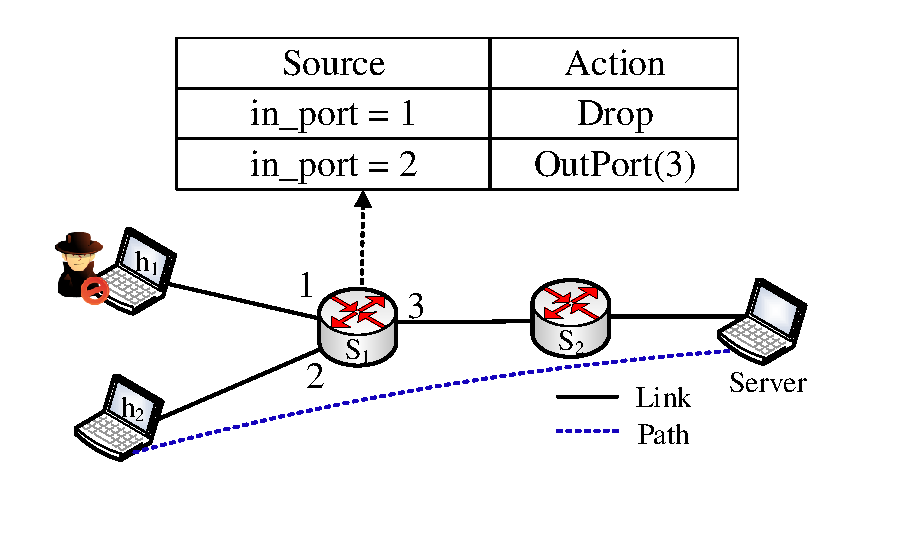
\includegraphics[width=3.4in]{Design/defense.pdf}
\vspace{-0.1in}
\caption{\small{An example of our defense.}}
\label{fig:mitigate}
\vspace{-0.2in}
\end{figure}



\section{Evaluation}

In this section, we introduce our experiment of \TheName{} and evaluate the effectiveness and overhead of our system. 

\subsection{Experiment Setup}
We use hardware SDN switch to test our approach. Floodlight, OpenFlow controller running our application, are deployed in an Intel Xeon Quad-Core CPU E5504 and 4GB RAM machine. We deploy two commercial hardware OpenFlow switch, EdgeCore AS4610-54T, in our hardware testbed, and the maximum transmitting rate of each port in the switch $R_m$ is 1 Gbps. We implement the attack in C code to generate the low-rate TCP attack with different $T$ and $L$. 

Figure~\ref{fig:topology} shows the topology of our testbed. $h_1$ generates the legitimate traffic as background traffic and $h_3$ receives the traffic. $h_2$ is generate the low-rate TCP attack traffic to $h_4$. The bandwidth of the link between $S_1$ and $S_2$ is overloaded and the queue of $S_1$ are congested for the period burst packet. The TCP flows affected seriously by low-rate TCP attack.

\begin{figure}
\vspace{-0.1in}
\centering
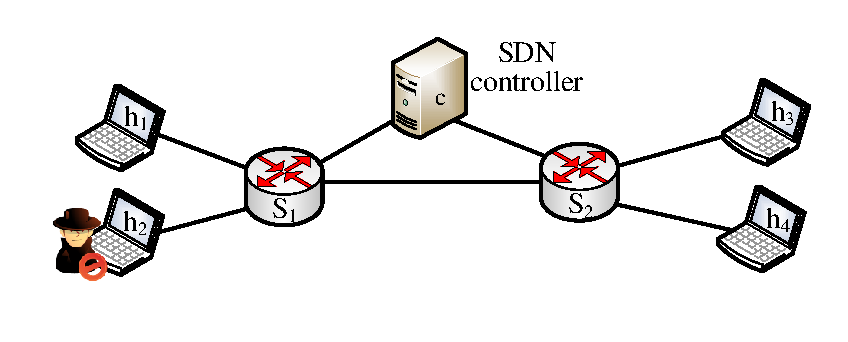
\includegraphics[width=3.4in]{Evaluation/topology.pdf}
\vspace{-0.1in}
\caption{\small{The network topology of our testbed.}}
\label{fig:topology}
\vspace{-0.2in}
\end{figure}

\subsection{Accuracy and Robustness}

We first measure the period by analyzing the statistics obtained from the counters associated with the active ports. After obtaining the sequence of the rate, we use the thresholding method to obtain the binary signals and measure the period of the signals. If there exists the low-rate TCP attack in a port, the measured period will be a positive value. Otherwise, the measured period will be zero. We compare the measured period of signals with the period of the low-rate TCP attack and obtain the error of the measurement.

\begin{figure}
\vspace{0in}


\begin{minipage}[t]{0.49\linewidth}
\centering
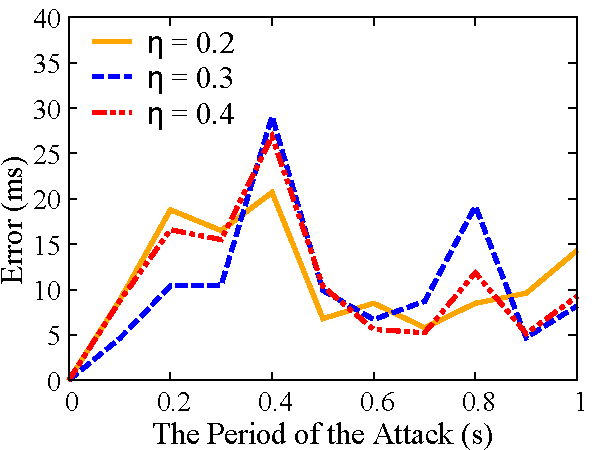
\includegraphics[width=1.7in]{Evaluation/period.pdf}
\caption{\small{Measurement Error}}
\label{fig:period}
\end{minipage}
\begin{minipage}[t]{0.49\linewidth}
\centering
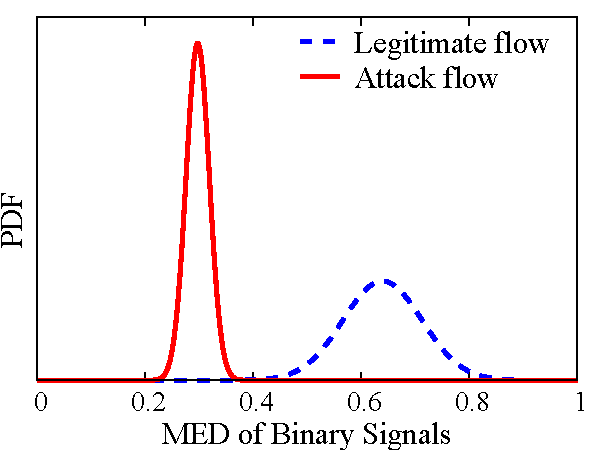
\includegraphics[width=1.7in]{Evaluation/distribution.pdf}
\caption{\small{PDF of MED}}
\label{fig:PDF}
\end{minipage}
\vspace{-0.2in}
\end{figure}

Figure~\ref{fig:period} shows the error of period measurement for various period values. We use Algorithm~\ref{alg:port_locate} to measure the period of the low-rate TCP attack. For the characteristics of the low-rate TCP attack, we consider $R $ = 1.1 Gbps. For the algorithm, we suppose that $T_{min}$  = 0.005s, $T_{max}$ = 0.64s, $\epsilon$ = 0.01. We set the period of the low-rate TCP attack from 0.1s to 1s. The periodicity of the flows can be detected and the period of the low-rate TCP attack is measured with the error ranging from 4 ms to 22 ms. Moreover, if none of the low-rate TCP attacks exist, the measured period and the error of the measurement will be zero. Furthermore, $T_s$ used for period measurement is also used for locating the attack hosts if the low-rate TCP attack exist.


For the appropriate threshold $\gamma$ to differentiate the legitimate and attack flows, the probability density function (PDF) of the MED between binary signals of potential flows and that of the affected ports is essential. Figure~\ref{fig:PDF} shows the PDF of MED for legitimate and attack traffic. The appropriate sampling period $T_s$ is obtained by the previous steps. We carry out an experiment to evaluate the MED between the binary signals of flow rule and that of the port. 
We consider the length of binary signals $N$=100, the period of the low-rate TCP attack $T$ is randomly chosen from [0.8,1.5], the burst length of the low-rate TCP attack $L$ is randomly chosen from (0, 0.4], and the burst rate is 1.1 Gbps. We generate 100 flows as legitimate flows. The MED of the attack flows basically ranges from 0.2 to 0.4 and the MED of the legitimate flows basically ranges from 0.4 to 0.8. In most cases, the MED of the attack flows is smaller than that of legitimate flows, because the majority of packets transmitted by the ports are the low-rate TCP attack packets. From Figure~\ref{fig:PDF}, A clear determination point (i.e. $MED$ = 0.4) can be obtained to differentiate attack flows from the legitimate flows.


Figure~\ref{fig:Performance} illustrates the performance of the binary classifier. We differentiate the attack flows by analyzing the similarity between the binary signals of the potential flows and that of ports. Considering the threshold $\gamma$ = 0.4. We sample the coming rate of ports for 5 $T_b$ measured before, classify them for the binary signals. We obtain MED between potential flows and the affected port by equation~(\ref{eq:euclidean_distance}) and differentiate the attack flows by $\gamma$. If the MED of a flow less than $\gamma$, we denote the flow as an attack flow. Otherwise, we denote the flow as a legitimate flow. We observe that attack flows detection have a recall rate of more than 90 percent and a false positive rate of less than 5 percent. Most of the attack flows are identified and the legitimate flows are not misidentified.


\begin{figure}
\vspace{0in}
\centering

\subfloat[\small{Recall rate}]{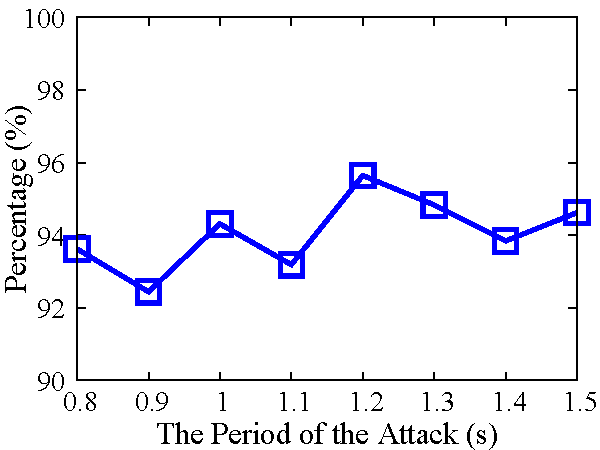
\includegraphics[width=1.7in]{Evaluation/recall.pdf}\label{fig:recall}}
\subfloat[\small{False positive rate}]{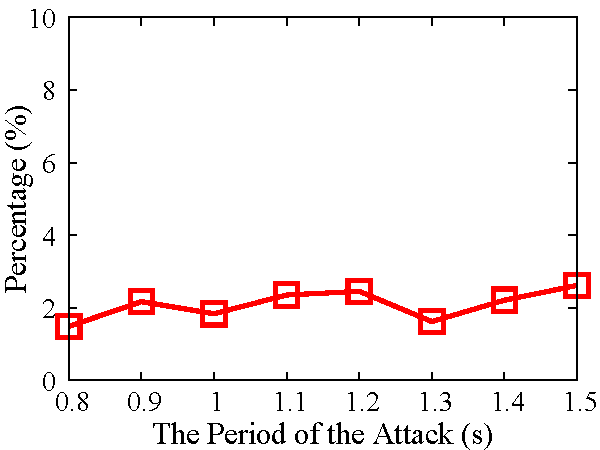
\includegraphics[width=1.7in]{Evaluation/false_positive.pdf}\label{fig:false_positive}}
\vspace{-0.1in}
\caption{\small{Performance.}}
\label{fig:Performance}
\vspace{-0.2in}
\end{figure}

\subsection{Evaluation of Defense Mechanism.} 
In this section, we show our evaluation on the effectiveness and overhead of \TheName{}. we first measure the throughput of a TCP flow with and without defense in the host. And then, we do the experiment for the CPU utilization with the low-rate TCP attacks with different periods.

\noindent \textbf{Effectiveness.}  We generate 100 TCP flows and they are transmitted by a port. we also generate the low-rate TCP attack traffic ($T$ = 210ms, $L$ = 90ms, $R$ = 1.1 Gbps) transmitted by the port. Figure~\ref{fig:throughput} shows a TCP flow throughput with and without attack. We record the throughput of a TCP flow on the host for 30 seconds. Under the low-rate TCP attack, the throughput of the TCP flow is almost zero. The reason is that the low-rate TCP attack forces the TCP flow to cause retransmission continuously. With the defense of \TheName{}, the low-rate TCP attack is mitigated at access switch. Hence, the TCP flow has a throughput of 8 Mbps.

\noindent \textbf{Overhead.} To evaluate the overhead of our system, we report the CPU utilization of the controller. We launch the low-rate TCP attack with $T$ from 0.1s to 1s and the flooding DoS. Figure~\ref{fig:utilizaition} shows that the overhead of \TheName{} with various period values. The controller overhead is increased because of the decrease of the period. According to the Nyquist theorem, the upper bound of the sampling period for the low-rate TCP attack is $T/2$, which means $T_s$ needs to be low enough for the low period values. Thus, the low period of the low-rate TCP attack incurs high overhead for the controller. If the attack is the flooding attack, the detection will terminate with a sampling period of $T_{min}$. \TheName{} introduces an additional CPU utilization of 25 percent at most. Such overhead is acceptable for deploying our defense system.

\begin{figure}
\begin{minipage}[t]{0.49\linewidth}
\centering
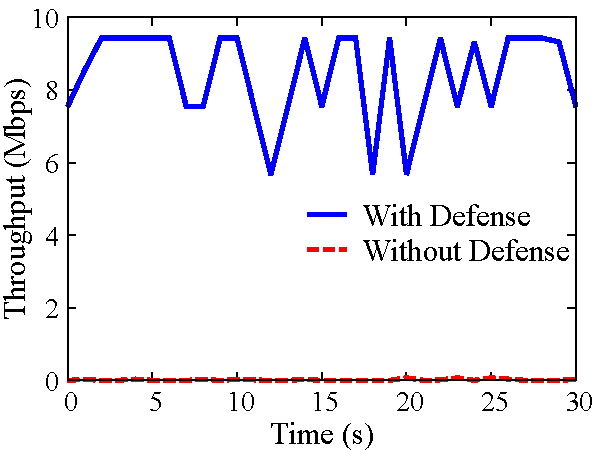
\includegraphics[width=1.7in]{Evaluation/throughput.pdf}
\caption{\small{The throughput with and without defense }}
\label{fig:throughput}
\end{minipage}
\begin{minipage}[t]{0.49\linewidth}
\centering
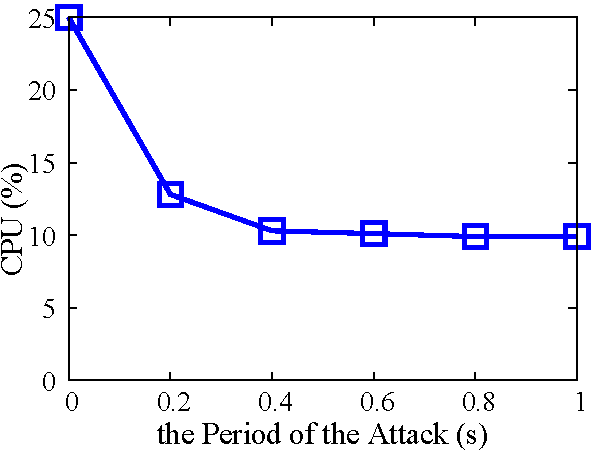
\includegraphics[width=1.7in]{Evaluation/utilizaition.pdf}
\caption{\small{CPU Utilization}}
\label{fig:utilizaition}
\end{minipage}
\vspace{-0.2in}
\end{figure}




\section{Related Work}

\noindent \textbf{Defending the low-rate TCP attack in Traditional IP Networks.} Several methods have been proposed to detect and mitigate the low-rate TCP attack in traditional IP networks. In \cite{b4}, the authors proposed a mechanism to dynamically detect and defend against the low-rate TCP attack. However, the mechanism fails to locate the source. In addition, the sampling period is a fixed value before working, which means failing to detect the low-rate TCP attack whose periods is smaller than the sampling periods, and the machine only works in the switches deploying it. In \cite{b5}, The author proposed four alternatives to defend the low-rate DoS attack against application servers. The approaches randomize the server operation to rearrange the positions in the incoming queues of applications for eliminating possible vulnerabilities due to predictable behaviors. In the frequency field, the sum of Low-Frequency Power spectrum (SLFP) \cite{b6} and cumulative amplitude spectrum (CAS) \cite{b7} have good performance on defending the low-rate TCP attack. Shrew Attack Protection (SAP) \cite{b8} is a port-based approach through the fair drop rate controller, and it prevents the victims from consecutive packet drops. \cite{b17} introduces randomization on TCP RTO to defense the low-rate TCP attack. 


\noindent \textbf{Defending DoS in SDN.} Bohatei \cite{b9} is a flexible and elastic approach based on SDN, and many types of known DDoS, e.g., SYN flood, DNS amplification, UDP flood, elephant flow, are inefficient for the victims with the system. Through the flow volume feature and the flow-rate asymmetry feature, the authors proposed adaptive methods to locate the potential victims and suspicious attackers on SDN's flow monitoring capability. \cite{b10},\cite{b12},\cite{b13},\cite{b15},\cite{b18} are proposed to defend SDN DoS attacks that exhaust control-data plane bandwidth, computational resources, and flow table. In [14], with the entropy-based method, SVM classifier, and mitigation agent in SDN, the network is protected from DDoS attacks. SPIFFY \cite{b16} introduces SDN to the defense of link-flooding attacks. ProDefense \cite{b11} solves the problem that traffic threshold for DDoS detection vary for existing SDN-based solutions and utilizes a distributed controller platform for load balancing and failure tolerance improvement. Although the existing defense approaches for DoS are deployed, the low-rate TCP attack may influence the hosts.


\section{Conclusions}
In this paper, we present \TheName to adaptive detect and defend against low-rate TCP attacks in SDN. We present the model of the low rate TCP attack. And then we design and implement a detection mechanism which takes advantage of periodicity and MED to detect the low rate TCP attack in SDN. We show that the detection is accurate and effective in identifying the attack flows. When the low-rate TCP attack is present, we install flow rule to defend the identified attack hosts in the access switch for the minimum influence of the attack due to the advantage of SDN. Experiments in a real SDN testbed consisting of commercial hardware switches demonstrate the accuracy and effectiveness of \TheName.

\begin{thebibliography}{00}
\bibitem{b1} Zhang C, Cai Z, Chen W, et al. Flow level detection and filtering of low-rate DDoS[J]. Computer Networks, 2012, 56(15): 3417-3431.
\bibitem{b2} Zhang Y, Mao Z M, Wang J. Low-Rate TCP-Targeted DoS Attack Disrupts Internet Routing[C]//NDSS. 2007.
\bibitem{b3} Chen Y, Hwang K, Kwok Y K. Filtering of shrew DDoS attacks in frequency domain[C]//Local Computer Networks, 2005. 30th Anniversary. The IEEE Conference on. IEEE, 2005: 8 pp.-793.
\bibitem{b4} Sun H, Lui J C S, Yau D K Y. Defending against low-rate TCP attacks: Dynamic detection and protection[M]. IEEE, 2004.
\bibitem{b5} Maciá-Fernández G, Rodríguez-Gómez R A, Díaz-Verdejo J E. Defense techniques for low-rate DoS attacks against application servers[J]. Computer Networks, 2010, 54(15): 2711-2727.
\bibitem{b6} Wei W, Dong Y, Lu D, et al. A novel mechanism to defend against low-rate denial-of-service attacks[C]//International Conference on Intelligence and Security Informatics. Springer, Berlin, Heidelberg, 2006: 261-271.
\bibitem{b7} Chen Y, Hwang K. Collaborative detection and filtering of shrew DDoS attacks using spectral analysis[J]. Journal of Parallel and Distributed Computing, 2006, 66(9): 1137-1151.
\bibitem{b8} Chang C W, Lee S, Lin B, et al. The taming of the shrew: mitigating low-rate TCP-targeted attack[J]. IEEE Transactions on Network and Service Management, 2010, 7(1): 1-13.
\bibitem{b9} Fayaz S K, Tobioka Y, Sekar V, et al. Bohatei: flexible and elastic DDoS defense[C]// Usenix Conference on Security Symposium. USENIX Association, 2015:817-832.
\bibitem{b10} Xu Y, Liu Y. DDoS attack detection under SDN context[C]//INFOCOM 2016-The 35th Annual IEEE International Conference on Computer Communications, IEEE. IEEE, 2016: 1-9.
\bibitem{b11} Bawany N Z, Shamsi J A, Salah K. DDoS attack detection and mitigation using SDN: methods, practices, and solutions[J]. Arabian Journal for Science and Engineering, 2017, 42(2): 425-441.
\bibitem{b12} Shang G, Zhe P, Bin X, et al. FloodDefender: Protecting data and control plane resources under SDN-aimed DoS attacks[C]//INFOCOM 2017-IEEE Conference on Computer Communications, IEEE. IEEE, 2017: 1-9.
\bibitem{b13} Xu T, Gao D, Dong P, et al. Defending against new-flow attack in sdn-based internet of things[J]. IEEE Access, 2017, 5: 3431-3443.
\bibitem{b14} Hu D, Hong P, Chen Y. FADM: DDoS Flooding Attack Detection and Mitigation System in Software-Defined Networking[C]//GLOBECOM 2017-2017 IEEE Global Communications Conference. IEEE, 2017: 1-7.
\bibitem{b15} Yang X, Han B, Sun Z, et al. Sdn-based ddos attack detection with cross-plane collaboration and lightweight flow monitoring[C]//GLOBECOM 2017-2017 IEEE Global Communications Conference. IEEE, 2017: 1-6.
\bibitem{b16} Kang M S, Gligor V D, Sekar V. SPIFFY: Inducing Cost-Detectability Tradeoffs for Persistent Link-Flooding Attacks[C]//NDSS. 2016.
\bibitem{b17} Yang G, Gerla M, Sanadidi M Y. Defense against low-rate TCP-targeted denial-of-service attacks[C]//Computers and Communications, 2004. Proceedings. ISCC 2004. Ninth International Symposium on. IEEE, 2004, 1: 345-350.
\bibitem{b18} Zhang M, Bi J, Bai J, et al. FloodShield: Securing the SDN Infrastructure Against Denial-of-Service Attacks[C]//2018 17th IEEE International Conference On Trust, Security And Privacy In Computing And Communications/12th IEEE International Conference On Big Data Science And Engineering (TrustCom/BigDataSE). IEEE, 2018: 687-698.
\bibitem{b19} https://www.wired.com/story/github-ddos-memcached/
\bibitem{b20} Kuzmanovic A, Knightly E W. Low-rate TCP-targeted denial of service attacks: the shrew vs. the mice and elephants[C]//Proceedings of the 2003 conference on Applications, technologies, architectures, and protocols for computer communications. ACM, 2003: 75-86.
\bibitem{b21} Zhang Y, Mao Z M, Wang J. Low-Rate TCP-Targeted DoS Attack Disrupts Internet Routing[C]//NDSS. 2007.
\bibitem{b22} Kwok Y K, Tripathi R, Chen Y, et al. HAWK: Halting anomalies with weighted choking to rescue well-behaved TCP sessions from shrew DDoS attacks[M]//Networking and mobile computing. Springer, Berlin, Heidelberg, 2005: 423-432.
\bibitem{b23} Shin S W, Porras P, Yegneswara V, et al. Fresco: Modular composable security services for software-defined networks[C]//20th Annual Network \& Distributed System Security Symposium. NDSS, 2013.
\bibitem{b24} Zheng J, Li Q, Gu G, et al. Realtime DDoS Defense Using COTS SDN Switches via Adaptive Correlation Analysis[J]. IEEE Transactions on Information Forensics and Security, 2018, 13(7): 1838-1853.


\end{thebibliography}

\end{document}
